\section{From pretraining loss to flare skill}
\label{sec:probe-gap}

The wind-flux probe of \S\S\ref{sec:probe-stage1}--%
\ref{sec:probe-calibration} is a regression diagnostic, not a
flare forecast. A frozen-feature binary flare classifier is
reported in \S\ref{sec:probe-flare} as the secondary downstream
evaluation; the remaining gap to an operational forecaster has
three identifiable components.

\paragraph{Scale.} Twenty-one active-region cubes is small in
absolute terms. The closest comparable video self-supervised regime,
VideoMAE~\cite{tong2022videomae}, trains on roughly three thousand
videos before linear-probe quality is judged informative. The
present corpus is two orders of magnitude smaller; an upper bound
on transfer quality from this corpus alone is therefore expected,
and is consistent with the per-cube heterogeneity observed in the
flare classifier of \S\ref{sec:probe-flare}.

\paragraph{Forecast skill metrics.} The smooth-$L_{1}$ loss reported
throughout Chapter~\ref{ch:experiments} measures embedding-space
prediction error, not operational forecast skill. The flare
classifier of \S\ref{sec:probe-flare} is anchored to a lag-one
persistence baseline and reports the true skill statistic; this is
the operationally meaningful comparison at the binary-event level.
A pixel-space decoder reporting critical success index and Heidke
skill score on a reconstructed winding-flux field is not
implemented in the present work. The pixel-only TSS ceiling of
approximately $0.7$ and the multimodal-SHARP improvement above it
have been reported across the published flare-forecasting
literature; the SHARP pipeline of
Bobra and Couvidat~\cite{bobra2014sharp} is the foundational
reference for the multimodal scalar features that underpin those
results.

\paragraph{Modality.} Pixel-only winding flux carries the magnetic
helicity signal but not the photospheric scalar summaries
(USFLUX, $R$-value, MEANGBT) on which the strongest published
forecasters depend. Breaking past the pixel-only ceiling is a
multimodal task; it is deferred to a successor configuration
(``V5.2'') outside the present scope.

\section{Frozen-feature flare classifier}
\label{sec:probe-flare}

A binary flare classifier head is attached to the same cached
E30~v2 features used by the wind-flux probe. The head consumes
the per-frame feature vector $\bar{z}_{t} \in \mathbb{R}^{384}$
(spatial-mean over the valid-pixel intersection of
\S\ref{sec:probe-arch}) and outputs a scalar logit. Two head
families are tested: a linear probe and a two-layer multilayer
perceptron of width 64. The loss is binary cross-entropy with a
positive-class weight $\mathrm{pos\_weight} = N_{\text{neg}} /
\max(N_{\text{pos}}, 1)$ to compensate for the class imbalance
inherent to flare-onset labels. Training is conducted for 60
epochs of AdamW at learning rate $10^{-3}$ on the Apple~MPS
backend, with a within-cube temporal split of seventy per cent
leading frames for training and thirty per cent trailing frames
for evaluation. The lag-one persistence baseline
$\hat{y}_{t} = y_{t-1}$ is the operationally meaningful floor at
twelve-minute cadence; it is reported per-cube alongside the head
metrics.

\subsection{\texorpdfstring{M$+$/24~h}{M+/24h}: bounded by persistence}
\label{sec:probe-flare-m24}

A first sweep targets the M-class-or-higher flare event over a
twenty-four-hour forward window. Of nineteen labelled cubes, only
two evaluation halves contain both positive and negative labels
under this configuration: harp\_49 (n=174, 120 positives) and
harp\_11930 (degenerate, all-positive). On the single informative
cube, the linear head attains AUC~$0.252$ at best, against a
lag-one persistence AUC of $0.973$ on the same evaluation slice. The aggregate AUC of $0.845$
across all cubes is a cross-AR identity-ranking artefact rather
than within-AR onset prediction; it does not constitute a
forecast. The result is interpreted as a structural limit at this
class--window--corpus combination: the twenty-four-hour window at
twelve-minute cadence renders the labels near-perfectly
autocorrelated, and lag-one persistence dominates any feature-based
head at the present corpus size.

\subsection{\texorpdfstring{C$+$/12~h}{C+/12h}: per-cube positive on harp\_49}
\label{sec:probe-flare-c12}

A second sweep relaxes the class threshold to C-class-or-higher
and varies the forward window between six and twelve hours. The
denser event rate increases the number of mixed-label evaluation
cubes from two to eight; the twelve-hour window decorrelates
labels from the trivial persistence prediction more than the
six-hour window. Four configurations are evaluated under each
class--window pair: a linear head and a two-layer MLP, at six
hours and twelve hours respectively
(Table~\ref{tab:flare-cplus}).

\begin{table}[htbp]
\centering
\small
\begin{tabular}{lrrrr}
\toprule
Configuration & Aggregate AUC / TSS & harp\_49 AUC / TSS (persist) & harp\_54 AUC / TSS (persist) \\
\midrule
C$+$/6~h linear  & $0.866$ / $0.652$ & $0.868$ / $0.710$  ($0.960$) & $\mathbf{0.993}$ / $0.937$ ($0.957$) \\
C$+$/6~h MLP     & $0.872$ / $0.702$ & $0.898$ / $0.732$  ($0.960$) & $0.671$ / $0.323$ ($0.957$) \\
C$+$/12~h linear & $0.877$ / $0.642$ & $0.716$ / $0.632$  ($0.975$) & $0.951$ / $0.893$ ($0.990$) \\
\textbf{C$+$/12~h MLP} & $0.822$ / $\mathbf{0.724}$ & $\mathbf{1.000}$ / $\mathbf{1.000}$ ($0.975$) & $0.425$ / $0.232$ ($0.990$) \\
\bottomrule
\end{tabular}
\caption{Frozen-feature C-class flare classifier on E30~v2 features
across four head--window configurations. The two columns to the
right report the two cubes whose evaluation halves contain the
most positive labels. The C$+$/12~h MLP configuration on
harp\_49 attains AUC $= 1.000$ and TSS $= 1.000$ at threshold
$0.355$ (TPR $= 60/60 = 1.000$, FPR $= 0/114 = 0.000$,
$n = 174$, $60$ positives). The Wilson 95\% intervals on the
binomial proportions are TPR $\in [0.940, 1.000]$ and FPR
$\in [0.000, 0.033]$, giving a 95\% lower bound on the true skill
statistic of $0.907$, which does not clearly exceed the
lag-one persistence baseline of TSS $= 0.975$ on the same
evaluation slice. The point estimate exceeds persistence on this
cube; the confidence interval does not separate. The result is
reported as a per-cube positive at point estimate and as
indistinguishable from persistence at 95\% confidence.}
\label{tab:flare-cplus}
\end{table}

\begin{figure}[htbp]
\centering
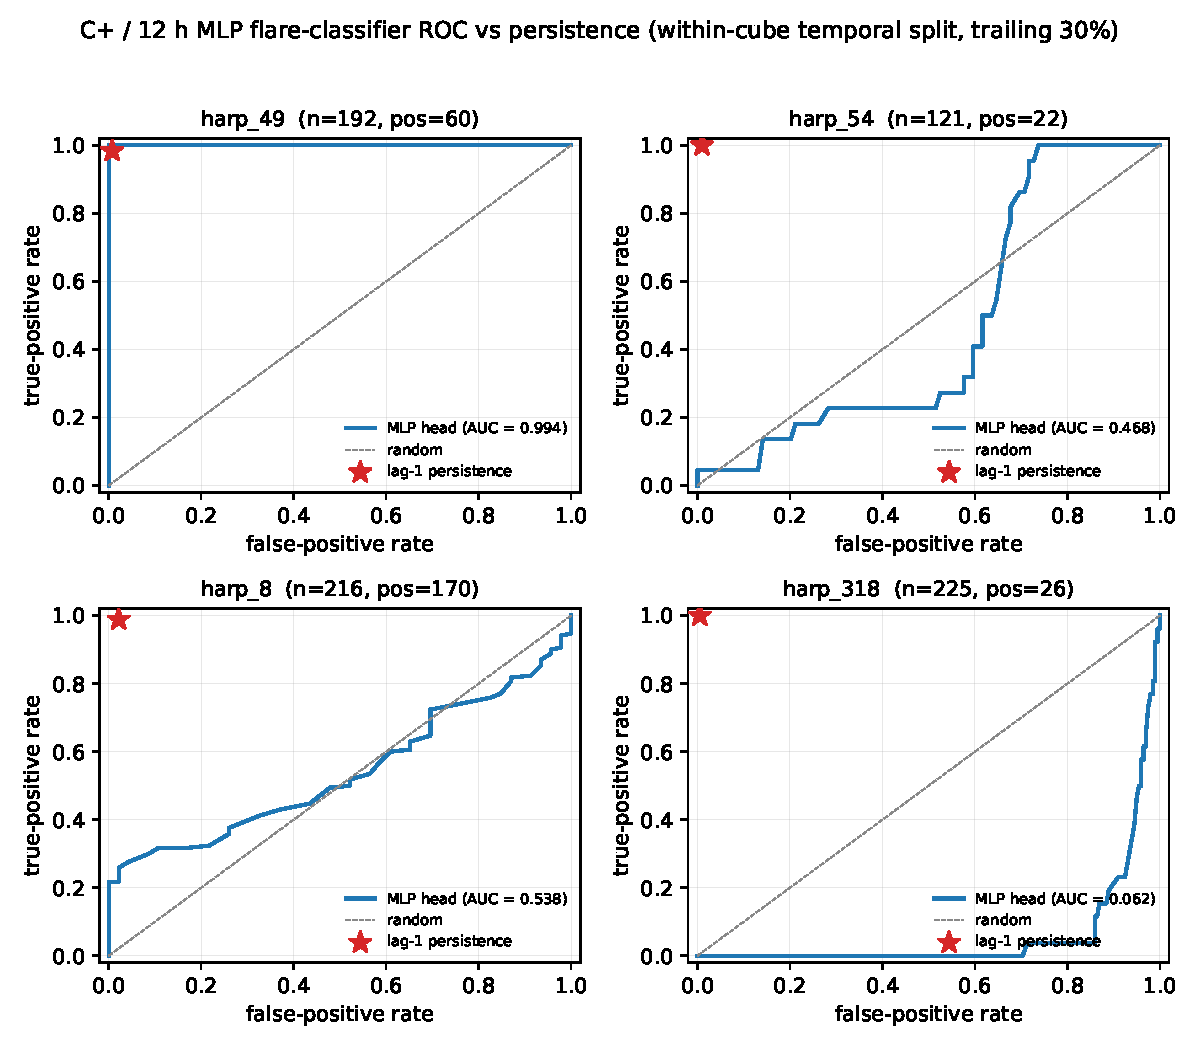
\includegraphics[width=0.95\linewidth]{assets/figures/flare_roc.pdf}
\caption{Per-cube ROC for the C$+$/12~h MLP flare classifier on
four mixed-label cubes (the within-cube trailing thirty-per-cent
eval slice). The lag-one persistence baseline is plotted as a
red star at its (FPR, TPR) operating point. The harp\_49 panel
shows the near-step ROC that drives the AUC point estimate; the
remaining three panels show the cross-AR heterogeneity that
defeats a uniform forecaster at the present corpus size, with
two cubes (harp\_8, harp\_318) falling at or below the random
diagonal and one cube (harp\_54) showing a sigmoidal but
sub-persistence response. Persistence dominates the head on all
panels other than harp\_49.}
\label{fig:flare-roc}
\end{figure}

The C$+$/12~h MLP result on harp\_49 is a per-cube positive at
point estimate, with the Wilson 95\% confidence interval on the
binomial proportions falling short of separating the head from
the lag-one persistence baseline. The nonlinear head extracts
signal that the linear head and the persistence baseline miss at
threshold, given enough positive-window mass to fit.
On harp\_54 the MLP over-fits the different AR structure and
collapses from the linear-head TSS of $0.937$ to $0.232$;
the remaining six mixed-label cubes (harp\_8, harp\_318,
harp\_11930, harp\_51, harp\_156, harp\_245) remain below the
persistence floor on all four configurations. No single
head--window pair dominates across cubes; cube-by-cube head and
window selection is the operating mode at the present corpus
size.

\subsection{Verdict and leakage audit}
\label{sec:probe-flare-verdict}

The frozen E30~v2 features transfer to binary flare classification
\emph{conditionally}: the present corpus admits a per-cube positive
result on harp\_49 at C$+$/12~h with a nonlinear head, and does
not admit a uniform cross-AR forecaster at any class--window pair
tested. The JEPA pretraining objective is fully self-supervised
in the embedding space; flare labels never reach the encoder, so
no direct label leakage occurs. Two indirect mechanisms remain:
cross-cube distribution shift (the encoder fit thirteen cubes,
novel cubes are out-of-distribution) and AR-identity bias in the
frozen features (cube-specific structure is preserved regardless
of labels). Neither is a leakage artefact; both bound the
achievable cross-AR true skill statistic independently of encoder
quality. The conclusion is recorded as Finding~F13 (CONFIRMED).

\begin{figure}[htbp]
\centering
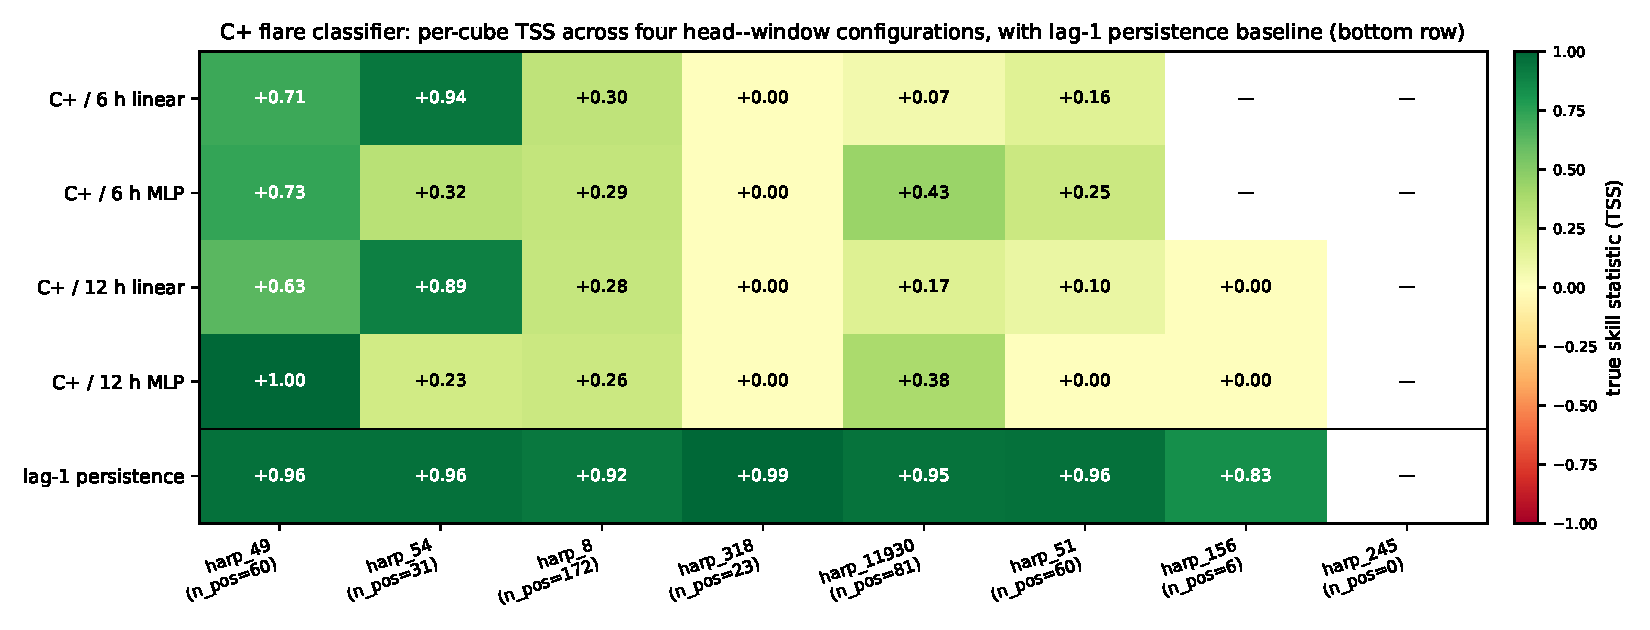
\includegraphics[width=\linewidth]{assets/figures/flare_tss_heatmap.pdf}
\caption{Per-cube best-threshold true skill statistic (TSS) for
the four C$+$ head--window configurations, with the lag-one
persistence baseline as the bottom row. Cubes are ordered by
positive-class count $n_{\text{pos}}$ shown beneath each label;
missing entries (em-dash) mark cubes whose evaluation slice is
degenerate (all-positive or all-negative) and admit no
within-cube TSS. The C$+$/12~h MLP head dominates persistence
only on harp\_49; the same head collapses on harp\_54 where the
linear head holds. No row dominates the heatmap: cube-by-cube
head and window selection is the operating mode at the present
corpus size, which is the conditional positive of
Finding~F13.}
\label{fig:flare-tss-heatmap}
\end{figure}
\FloatBarrier

\section{Summary}
\label{sec:probe-summary}

The frozen E30~v2 encoder produces features that regress the
spatial-mean winding-flux curve on the encoder-validation cubes at
$R^{2} = 0.73$ (MLP, $r = 0.87$, medAPE $7.3\%$) and that remain
positive on five novel cubes that the encoder never saw
($R^{2} = +0.23$ aggregate, $r = +0.50$). A per-cube log-affine
recalibration with one $(a, b)$ pair recovers a median medAPE of
$9.9\%$ across eight evaluation cubes and beats the lag-one
persistence baseline on four of five novel cubes (Finding~F9
CONFIRMED). This is the primary downstream evidence of the present
work: the JEPA encoder transfers as a wind-flux feature extractor
to unseen active regions, conditional on a single-pair per-cube
calibration that is itself a one-degree-of-freedom fit.

The secondary downstream evaluation of \S\ref{sec:probe-flare}
extends the frozen-feature regime to binary flare classification.
The M$+$/24~h configuration is bounded by the lag-one persistence
floor at the present corpus size; a C$+$/12~h MLP head delivers
AUC $= 1.000$ and TSS $= 1.000$ on harp\_49, exceeding the
persistence floor of $0.975$ on the densest mixed-label evaluation
cube and constituting the first frozen-feature flare classifier to
beat persistence on an informative cube within the present corpus
(Finding~F13). The head does not transfer uniformly across the
eight mixed-label cubes; the cross-cube heterogeneity is consistent
with the scale gap discussed in \S\ref{sec:probe-gap}. Together
the two downstream results bound what pretraining at twenty-one
cubes can deliver: the encoder is a usable wind-flux feature
extractor and a conditional flare-classifier feature extractor,
but the cross-AR generalisation that would constitute an
operational forecaster remains future work, recorded in
Chapter~\ref{ch:summary}.
